\section{La carte SABRE Lite}

Afin d'effectuer un profilage réaliste, nous allons réaliser notre portage et
nos expérimentations sur un système embarqué répandu dans l'industrie, notamment
dans le monde de l'automobile. Il s'agit d'une carte SABRE Lite
\cite{_i.mx_2014} de Freescale. Il est important de bien connaître le matériel
utilisé pour pouvoir comprendre ses limites et les résultats des mesures.

\subsection{Caractéristiques techniques}

La carte SABRE Lite embarque un processeur i.MX 6, basé sur le
processeur ARM Cortex A9 MPCore (Figure \ref{fig:archi}). Il s'agit d'un
processeur quad-core cadencé à 1 GHz, disposant de caches L1 de 32 Ko ainsi que
d'un cache L2 de 1 Mo partagé pour les quatre coeurs. La carte dispose également
de 1 Go de mémoire vive (DDR3). Le contrôleur mémoire contient plusieurs
compteurs permettant la mesure de l'activité mémoire qui seront utilisés dans la
phase de profilage détaillée dans la suite de ce rapport. Une puce de mémoire
flash SPI de 2 Mo contenant un code de boot est aussi présente.

\begin{figure}[H]
\centering
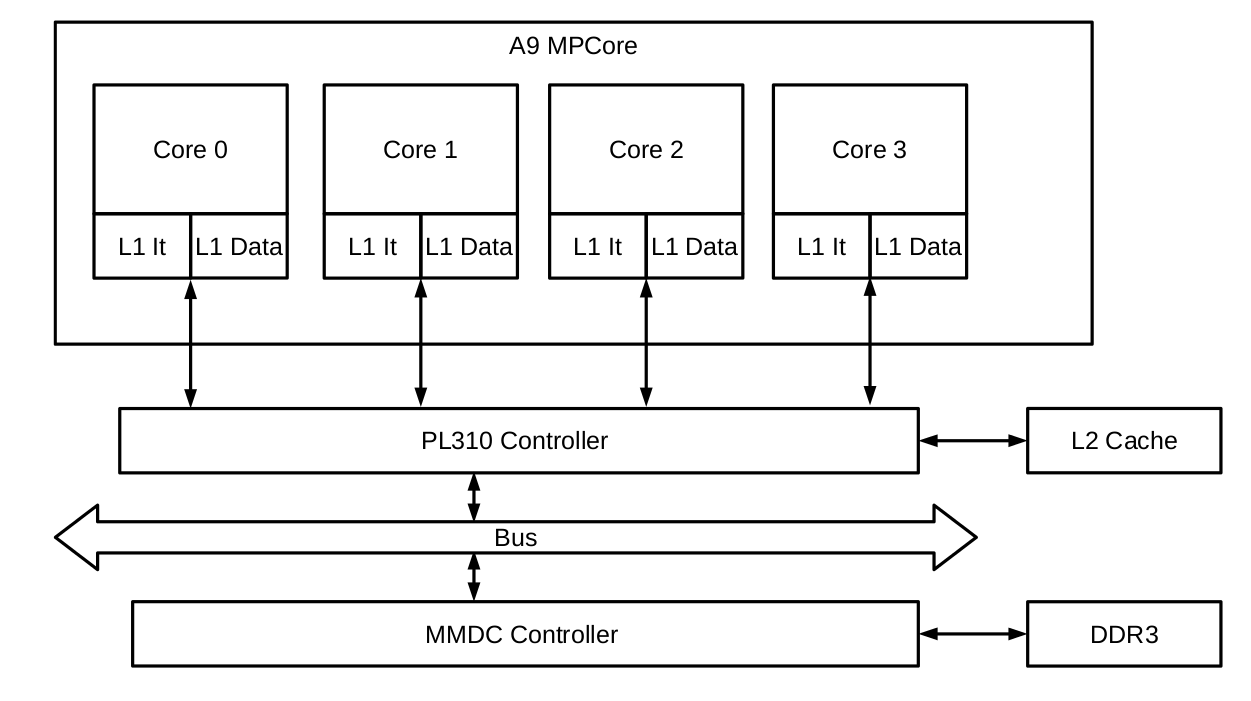
\includegraphics[scale=0.3]{include/sabrelite_archi.png}
\caption{Architecture de la carte SABRE Lite}
\label{fig:archi}
\end{figure}

\paragraph{}
Le système ne dispose pas de périphérique de stockage de masse interne mais de
ports permettant l'ajout de périphériques de stockage externes :
\begin{itemize}
\renewcommand{\labelitemi}{$\bullet$}
\item un port SATA pour connecter un disque dur ou un SSD,
\item deux ports USB 2.0,
\item un port microUSB 2.0 supportant la norme OTG, afin de permettre au 
  périphérique de commander les échanges vers la carte,
\item un port SD et un port microSD.
\end{itemize}

\paragraph{}
La carte dispose également d'un port Ethernet pour se connecter au réseau, ainsi
que d'un port UART, permettant une liaison série avec un ordinateur. Cette
liaison série sera notamment utilisée lors de la configuration de la carte. La
carte embarque également les ports suivants :
\begin{itemize}
\renewcommand{\labelitemi}{$\bullet$}
\item HDMI
\item microphone et casque
\item GPIO/I2C
\item PCIe
\item LVDS (Low-Voltage Differential Signaling)
\item caméra
\end{itemize}

\subsection{Image système}
Afin de rendre la carte utilisable, il est bien entendu nécessaire d'y installer
un système d'exploitation. Il est possible de booter la carte de deux manières :
\begin{itemize}
\renewcommand{\labelitemi}{$\bullet$}
\item via le port microUSB OTG,
\item via la mémoire flash interne
\end{itemize}
Le mode de boot est contrôlé par un interrupteur sur la carte. Dans notre cas,
nous allons utiliser le code de boot préchargé dans la mémoire flash interne
pour ensuite charger l'image présente sur une carte microSD et démarrer sur
cette dernière.

\subsubsection{Construction de l'image}
Afin de construire l'image système pour la carte SABRE Lite, nous avons
utiliser la suite d'outils du projet Yocto\cite{hallinan_create_2015}. Il s'agit
d'un projet géré par la Linux Foundation et plusieurs grandes entreprises du
monde de l'embarqué (Intel, Texas Instruments, Huawei, ...). Cette suite permet
notamment la construction d'images Linux personnalisées pour systèmes embarqués.
La construction se fait par couches (\texttt{layers}), chacune représentant un
ensemble logique de recettes (\texttt{recipes}). Une recette est une suite
d'instructions détaillant des étapes de construction (dépendance à d'autres
recettes, origine des sources, paquets à installer, ...).

\paragraph{} Après avoir concocté les couches et les recettes nécessaires à la
construction de l'image système (l'ajout d'un client \texttt{ssh} à une image
minimale dans notre cas), l'outil \texttt{bitbake}\cite{purdie_bitbake_????}
de la suite Yocto exécute toutes les recettes. Ce dernier construit entièrement
l'image pour le système ciblé, notamment en téléchargeant les sources de tous
les paquets et en les recompilant un à un. Des partitions (image kernel
\texttt{uImage}, rootfs), ainsi qu'une image pour carte SD contenant ces
dernières, sont alors générées.

\subsubsection{Déploiement de l'image}
L'image se déploit très simplement sur une carte SD, soit en copiant via un
outil tel que \texttt{dd} l'image pour carte SD générée, soit en partitionnant
la carte SD (Figure \ref{partSD}) et en copiant les partitions générées une à
une \cite{angolini_yocto_2014}.

\begin{figure}
  \centering
  \begin{tabular}{|c|c|c|c|}
    4 Mio & 8 Mio & ROOTFS\_SIZE & 4 Mio \\
    \hline
    réservé au bootloader & kernel & rootfs & non \\
    (non partitionné) & (uImage) & & partitionné \\
  \end{tabular}
  \caption{Partitionnement de la carte SD}
  \label{partSD}
\end{figure}

\paragraph{} Maintenant que la carte SD est prête, il faut configurer notre
SABRE Lite afin de booter sur celle-ci. Pour cela, nous allons tout d'abord
démarrer sur le mémoire flash SPI qui contient un code de boot
(\texttt{U-Boot}\cite{denk_denx_2015}) préchargé. Sur cet environnement de
boot, il est possible de gérer les périphériques, de configurer la séquence de
boot, etc... \\
Dans notre cas, nous avons seulement :
\begin{itemize}
\renewcommand{\labelitemi}{$\bullet$}
\item sélectionné le port microSD, 
\item configuré les arguments de boot du kernel Linux (nom et débit de la
  console, chemin vers le \textit{rootfs}, \texttt{rootwait} pour que le kernel
  attende la détection de la carte SD),
\item chargé l'image kernel (\texttt{uImage}) en mémoire,
\item et enfin booté à l'adresse de l'image kernel.
\end{itemize}
(Figure \ref{ubootcmds})

\begin{figure}[H]
  \centering
  \begin{lstlisting}[language=bash, frame=single, basicstyle=\scriptsize]
    mmc dev 1
    fatload mmc 1:1 0x10800000 uImage
    setenv bootargs console=ttymxc1,115200 rootwait root=/dev/mmcblk0p2
    bootm
  \end{lstlisting}
  \caption{Commandes de configuration du U-Boot}
  \label{ubootcmds}
\end{figure}

\paragraph{}
Les différents essais de déploiement d'images que nous avions nous mêmes créées
ont systématiquement échoué lors du boot, la carte se bloquant lors du boot
du kernel, après avoir été chargé en mémoire. Faute de temps, nous n'avons pu
résoudre ce problème et nous sommes donc tournés vers une image déjà créée et
fonctionnelle, afin de nous concentrer sur la suite du projet, à savoir le
portage de l'application ainsi que le profilage sur la carte.
